\chapter{Evaluation} 
This chapter presents an evaluation of the initial results from the collected data focusing on statistics relating to
developmental trajectories in order to identify potential developmental indices. These findings serve as the
foundation
for the feature selection used in training the explainable boosting machine. Features that demonstrate strong
performance here may also be identified as important by the EBM. The following questions will be addressed in this
section:

\begin{enumerate}
    \item Which measures show an overall developmental trajectory across JLPT levels?
    \item Which features significantly discriminate between proficiency levels, and is a developmental trajectory
    apparent across these levels?
\end{enumerate}

\section{Complexity Measures}

Many of the complexity measures demonstrated trends that correspond to increasing proficiency. However, the patterns
varied across measures. Some showed a consistent increase,while others
decreased, or plateaued at the
higher levels. Notably, most measures were unable to distinguish between the N1 and native speaker (NS) groups.

Statistical analyses were conducted using ANOVA to test for significance, followed by Tukey's HSD test to identify
significant pairwise differences between adjacent proficency levels.

\subsection{Syntactic Complexity Measures}

%Sentence Length
    %discriminates between ajacent proficency levels.
%Clause per Sent
    %*Statistically significant difference between all adjacent levels except N1 and NS

Many of syntactic measures failed to show significant differences between N1 and NS groups. This however is not
cause for concern as the Native speaker group is not actually part of the JLPT scale and is used as a benchmark to
compare how close to native like speech the other learner's are. Therefore when it is mentioned that a measure
distinguished all adjacent levels this means all levels within the JLPT proficency scale not including the native
speaker group.
However several measures
such as sentence length, clauses per sentence, and coordinating clauses per sentence exhibited statistical significance
across most
adjacent proficency levels. These patterns are illustrated in Figures \ref{fig:sentLen}, \ref{fig:cpersent}, and
_____ respectively.

\begin{figure}[htbp]
    \centering
    \begin{minipage}{.48\textwidth}
        \centering
    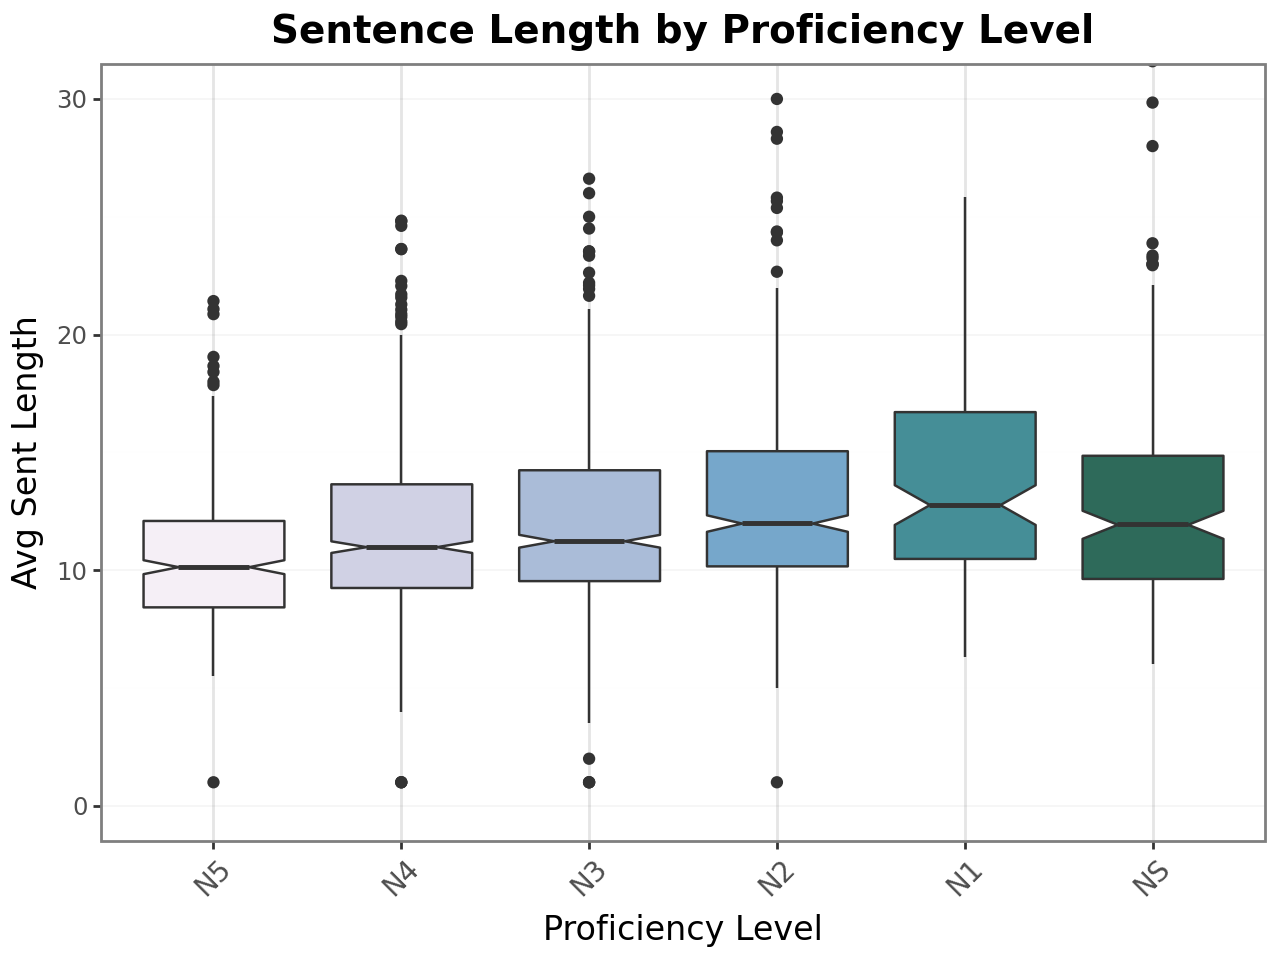
\includegraphics[scale=.3]{img/sentence_len}
    \caption[Average Sentence Length across JLPT levels]{Average Sentence Length across JLPT levels}
        \label{fig:sentLen}
    \end{minipage}
    \hfill
\begin{minipage}{.48\textwidth}
        \centering
        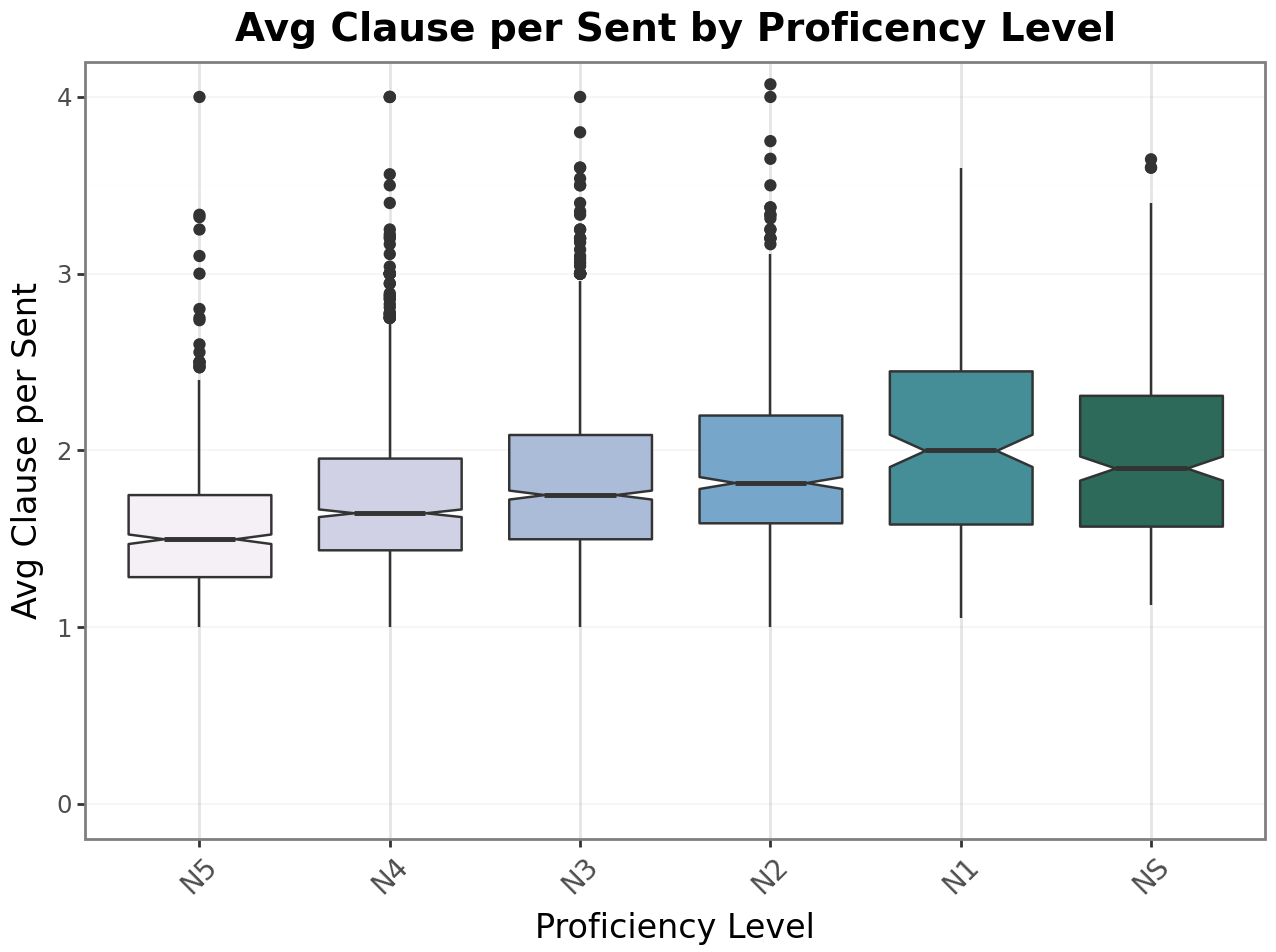
\includegraphics[scale=.3]{img/clausesSent}
        \caption[the ratio of clauses per sentence]{Plot showing the ratio of clauses per sentence}
\label{fig:cpersent}
\end{minipage}
    \end{figure}


\subsubsection{Length-Based Measures}

Length-based metrics capture the amount of syntactic material produced per unit (e.g. per sentence, per clause,
etc.) and are surface level-indications of syntactic complexity. Sentence length exhibited a general upward trend
across proficiency levels and was statistically significant at distinguishing across most adjacent levels, although
it failed to distinguish N1 from the NS group. This aligns
with
the idea that more advanced learners integrate more elements into a single sentence.

Noun phrase length and verb phrase length in contrast, were less informative. NP length remained relatively stable
and did not significantly differ across levels. Verb phrase length did show a weak upward trend but lacked
statistical significance to distinguish between the proficiency levels.

\subsubsection{Clause-Based Measures (Including Coordination/Subordination)}
Clause based measures focus on how learners structure and link clauses, capturing syntactic elaboration through
subordination and coordination.
%Clause Length
%    *N1 and N3 statistically significant difference observed
%    *slightly increases across levels.
%    *Could be influenced by tasks?. Try Removing SW1 and SW2 tasks

Clause length showed a slight
increase across proficiency levels, with a statistically significant difference in distinguishing between N1 and N3.
However, when the SW1 and SW2
tasks were removed, this measure distinguished between all adjacent upper proficiency levels, suggesting a at a
possible
task effect. increases in clause length were more pronounced at the advanced stages than at the beginner levels,
hinting at its potential in detecting finer gradiations of advanced proficiency.

%add other citations
Across prior studies on l2 syntactic development, a common finding is a decrease in coordination and an increase in
subordination with proficiency \citep{Vyatkina2012, Lu2010,Lu2011}. However, in the present data, this trend was not
entirely replicated. One reason may be the early introduction of subordinating conjunctions in Japanese L2
instruction such as 「から」(kara, \textit{because}) and 「けど」(kedo, \textit{but}) which are frequently used without
requiring transformation of verbs or deep syntactic embedding.

%Subordinate Clauses per Sent
    %statistically significance difference between N5 and N4 ,and then N1 and N3 but does not discriminate between the
%higher proficency
    %levels. Subordination is taught quite early to L2 speakers, could this be why?
%Subordinate Clause per clause
    %statistically significant difference between N5 and N4 and N4 and N3,
    %slight decrease across levels showing a prefernce for different clause types in the higher levels?

The measure of subordinate clauses per sentence showed a modest increase across proficiency levels and was
statistically significant in distinguishing lower levels(N5 vs N4) and non-adjacent upper levels (N3 vs N1). This
reflects developmental progression but not ina  linear fashion (see Figure~\ref{fig:SubclperS}).

In contrast, the ratio of subordinate clauses to total clauses showed a decreasing trend, with significant
differences observed between non-adjacent levels (N5 vs N3, N4 vs N2).  As shown in Figure~\ref{fig:SCperC}, this
suggests that lerners at higher proficiency levels may diversify their clause structures and shift toward more
coordination or other complex constructions.

\begin{figure}[htbp]
    \centering
    \begin{minipage}{.48\textwidth}
        \centering
    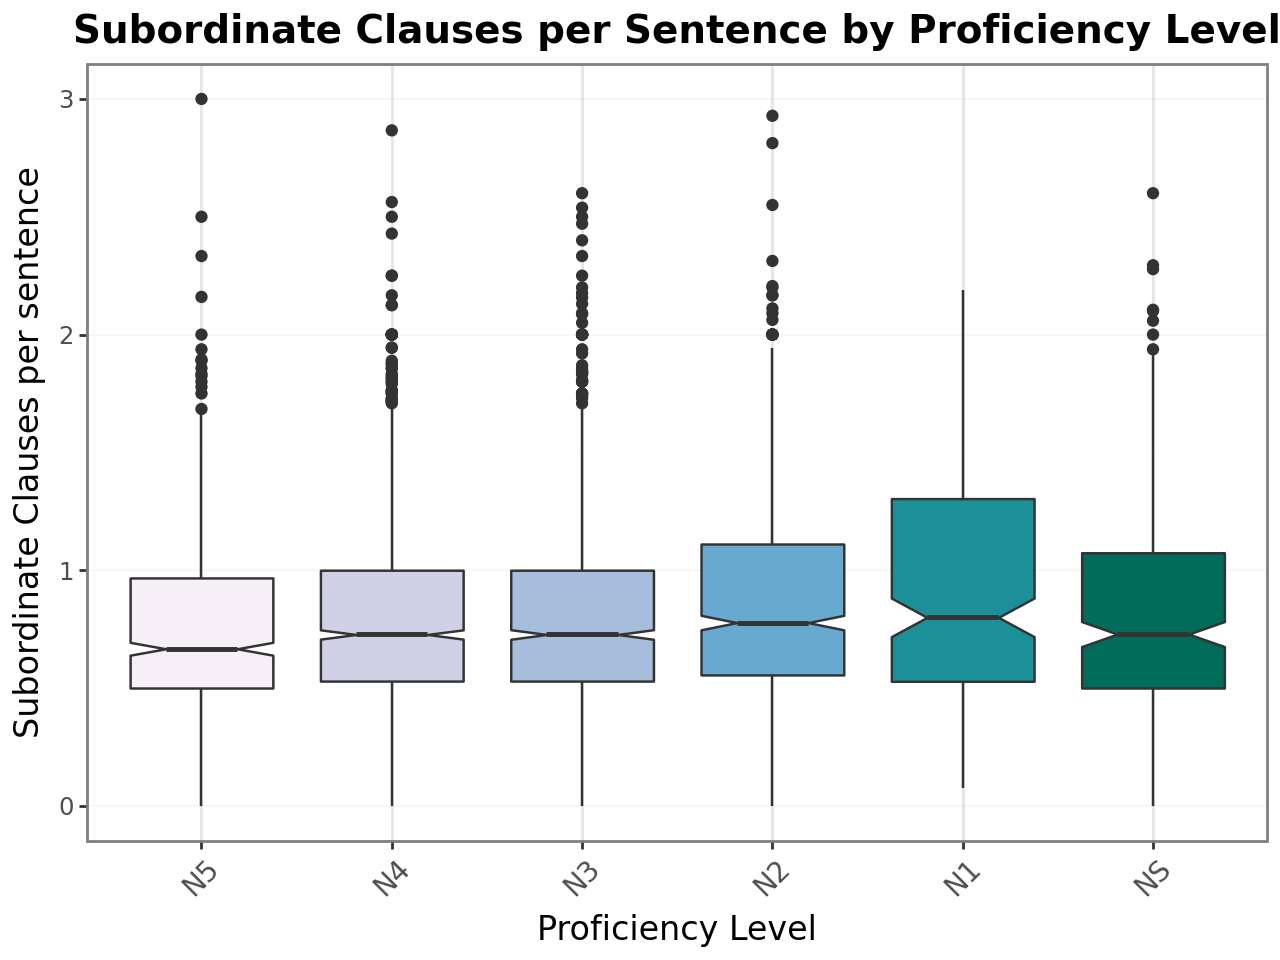
\includegraphics[scale=.3]{img/SCperS}
    \caption[Average subordinate clauses to sentences across JLPT levels]{Average subordinate clauses to sentences across JLPT levels}
        \label{fig:SubclperS}
    \end{minipage}
    \hfill
\begin{minipage}{.48\textwidth}
        \centering
        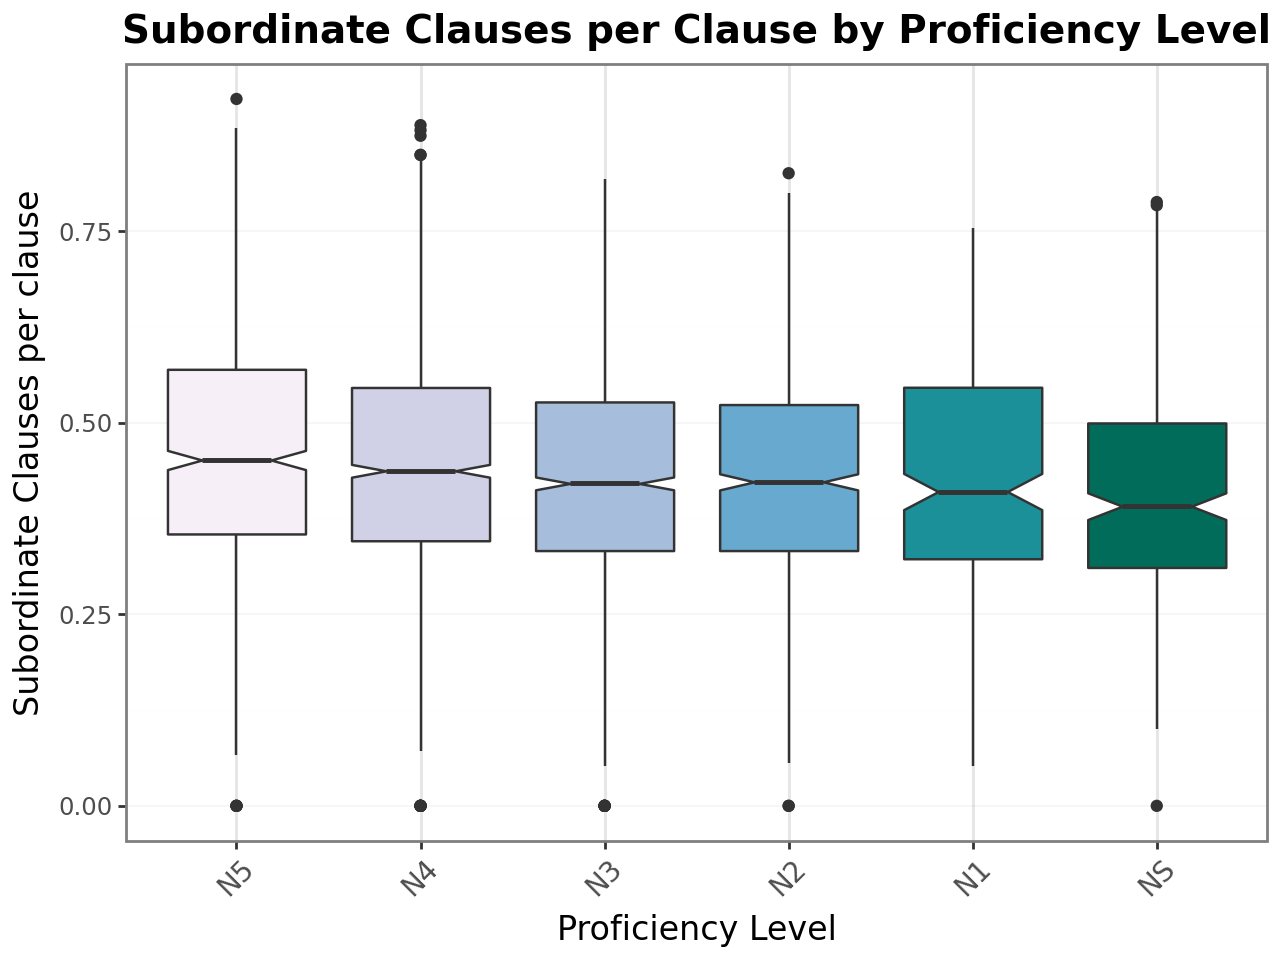
\includegraphics[scale=.3]{img/SCperC}
        \caption[Average subordinate clauses to clauses ratio across JLPT levels]{Average subordinate clauses to clauses ratio across JLPT levels}
\label{fig:SCperC}
\end{minipage}
    \end{figure}

%Coordinating Conjunction per Sentence
    %*Statistically significant in distinguishing all adjacent levels except N1 and NS group
    %*Also increases across prof levels, could be due to the fact that SC are taught first.
%Coordinating Conjunction per Clause
    %*increase across prof. levels
    %*Statistically significant between levels except N2 & N1 and N1 & NS
%Subordinating Clauses to Coordinate Clauses
%    *statistically significant for every other proficency level. ie. N5 & N3, N3 & N1, N2&N4
%    *variance also increases at the higher proficency levels but , maybe due to more CC being used?

Measures related to coordination showed strong developmental patterns. The number of coordinate clauses per sentence
increased across levels and significantly
distinguished all adjacent levels. This trend may reflect increased syntactic range at higher levels where
coordination is used stylistically or rhetorically, not just structurally (Figure~\ref{fig:CCperSent}).

Similarly, coordinate clauses per clause also increased with proficiency and distinguished most adjacent levels
except N2 - N1 (Figure~\ref{fig:CCperCl}). These findings contrast with typical L2 development models by maybe due
to the instructional sequence in Japanese, where simple subordinate forms are taught earlier and coordination
becomes more common as learners diversify their expression.

The ratio of subordinate clauses to
coordinate clauses further supports this shift. It showed statistically significant differnces between non-adjacent
levels (N5 vs N3, N3 vs N1) and increased variance at higher proficiency levels, possibly reflecting more
individualized or task-drive distribution of clause types.

\begin{figure}[htbp]
    \centering
    \begin{minipage}{.48\textwidth}
        \centering
    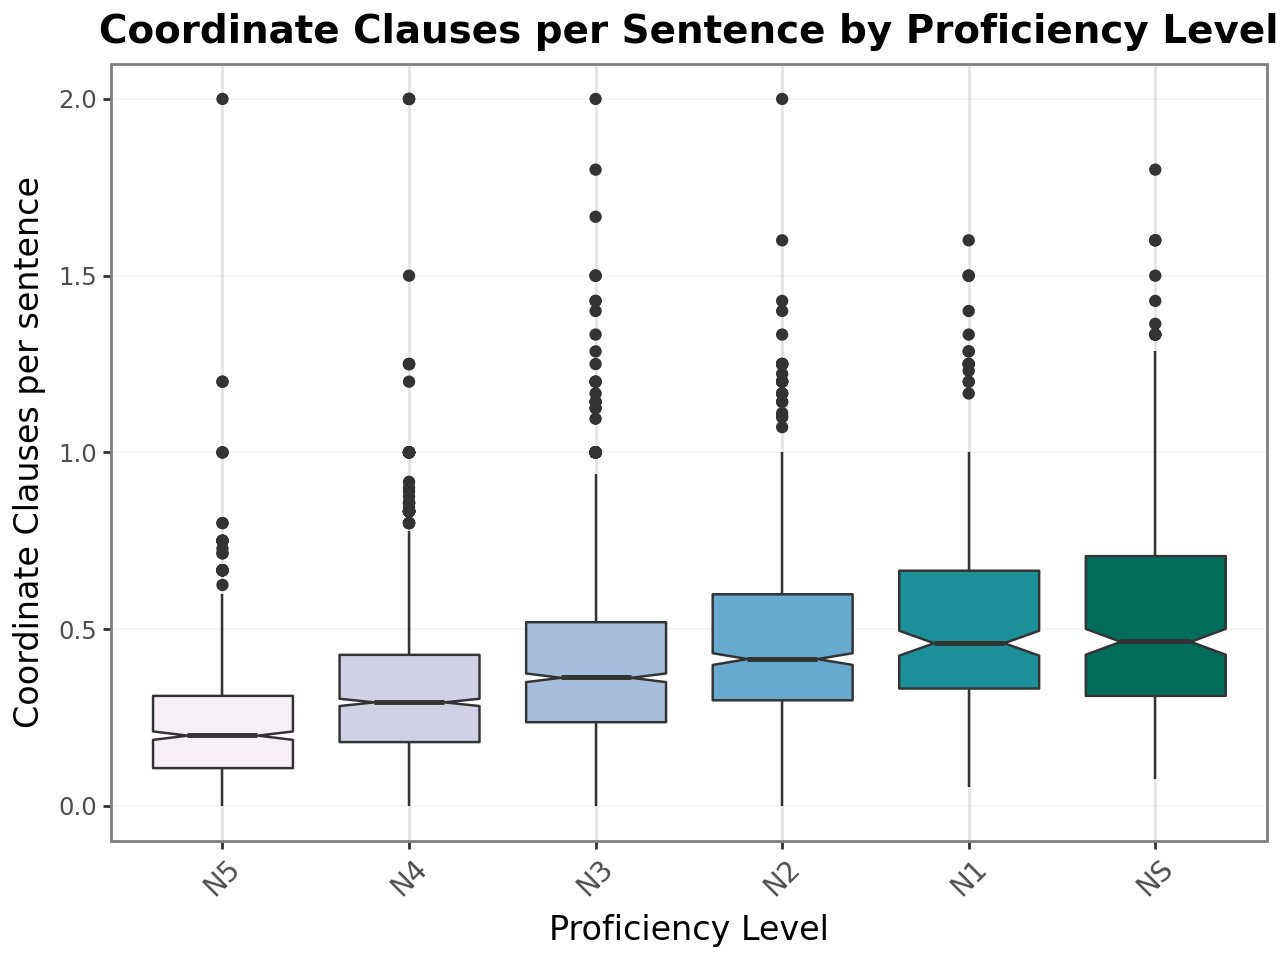
\includegraphics[scale=.3]{img/CCperSent}
    \caption[Average coordinate clauses to sentences across JLPT levels]{Average coordinate clauses to sentences across JLPT levels}
        \label{fig:CCperSent}
    \end{minipage}
    \hfill
\begin{minipage}{.48\textwidth}
        \centering
        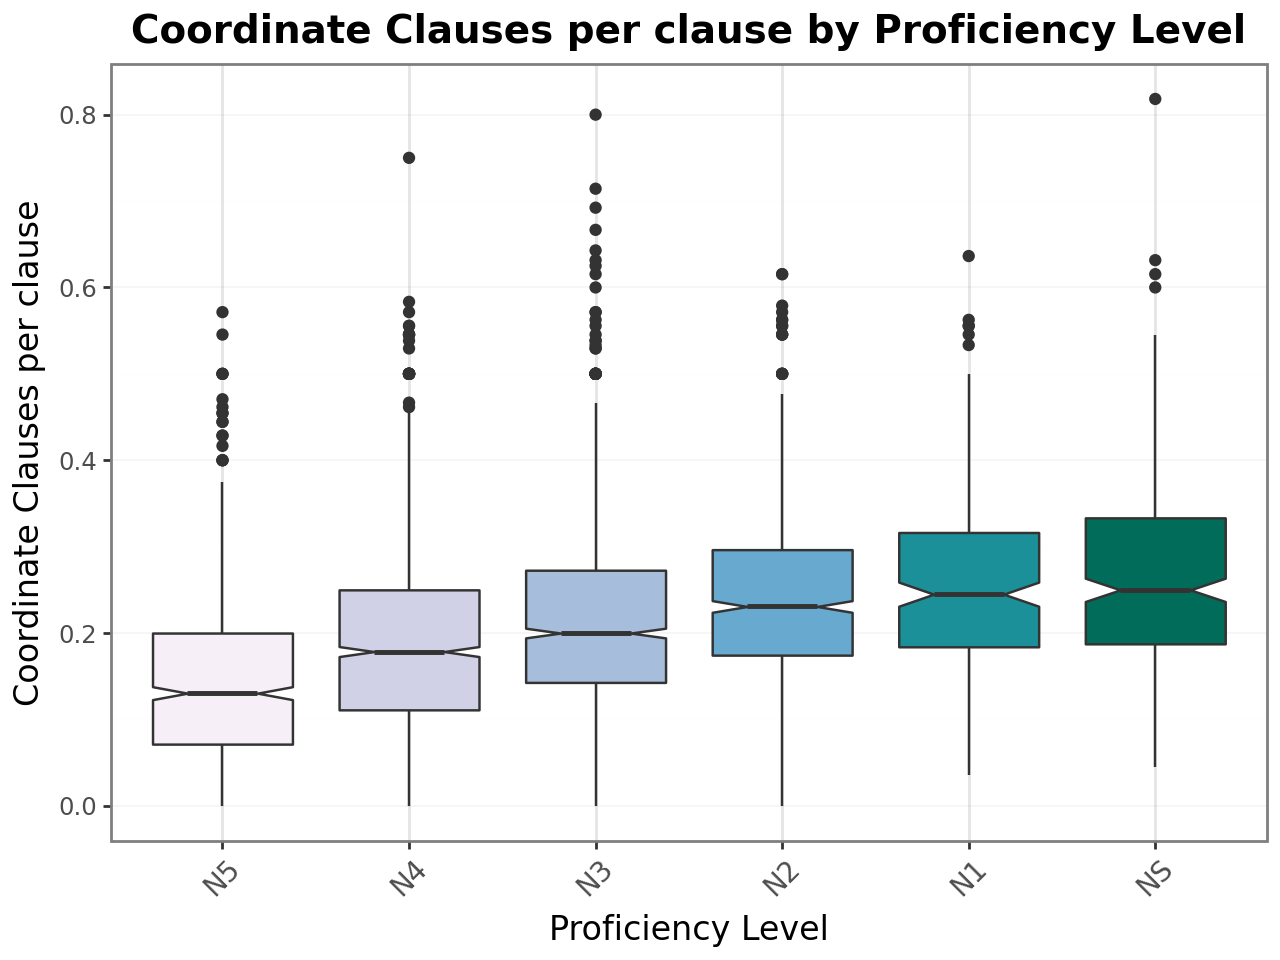
\includegraphics[scale=.3]{img/CCperC}
        \caption[Average coordinate clauses to clauses ratio across JLPT levels]{Average coordinate clauses to clauses ratio across JLPT levels}
\label{fig:CCperCl}
\end{minipage}
    \end{figure}

%CC Freq
    %no significant difference between any of the levels and no clear pattern...
%SC Frequency
    %*increases across levels
    %*Significant between n5&N4, N4&N3, N3&N2, N2 & NS
Normalized frequencies of subordinating and coordinating conjuctions were analyzed as a proxy measure as done in \citet{Vyatkina2012}, however, they showed mixed results. Subordinating conjunction frequecy increased across proficiency levels and showed statistically significant differences at lower levels (N5 vs. N4, N4 vs N3), reflecting early acquisition and frequent use. Coordinating conjunction frequency, however, did not show significant variation across levels and did not follow a clear developmental trend. This may be due to extraction limitations or the realtively sparse distribution of explicit coordinators in learner texts.

\subsubsection{Dependency-Based Measures}

Dependency-based measures provide a structural perspective on syntactic complexity by quantifying how syntactic
units are hierarchically and linearly related. Unlike length or clause-based measures, which capture surface level
elaboration, these metrics reflect the cognitive load and integration required to process or produce a sentence.
Both measures considered, Mean Dependency Distance (MDD) and Mean Hierarchical Distance (MHD), showed strong
associations with increasing proficiency and can be considered promising indicators of developmental progression.

%MDD
    %* Statistically significant between every other level as well as the higher proficency levels N3&N2 and N2&N1
    %*no significant between N1 and NS
    %*Increase across levels
As shown in Figure~\ref{fig:mdd}, MDD increased consistently across proficiency levels and was statistically
significant between most levels, including higher-level distinctions such as N3 vs. N2 and N2 vs. N1. The consistent
upward trajectory suggests that as learners become more proficient, they are able to manage longer dependency
relations, producing more integrated syntactic structures.

%MHD
%    *Increase across levels
%    *statistically significant between all adjacent levels except NS and N1

Similarly, MHD, depicted in Figure~\ref{fig:mhd}, also exhibited a steady increase with proficiency. It was
statistically significant across all adjacent levels. This measure captures the hierarchical depth of sentence
structure, and its strong performance across levels supports the idea that syntactic embedding becomes more complex
and frequent as learners advance.

\begin{figure}[htbp]
    \centering
    \begin{minipage}{.48\textwidth}
        \centering
    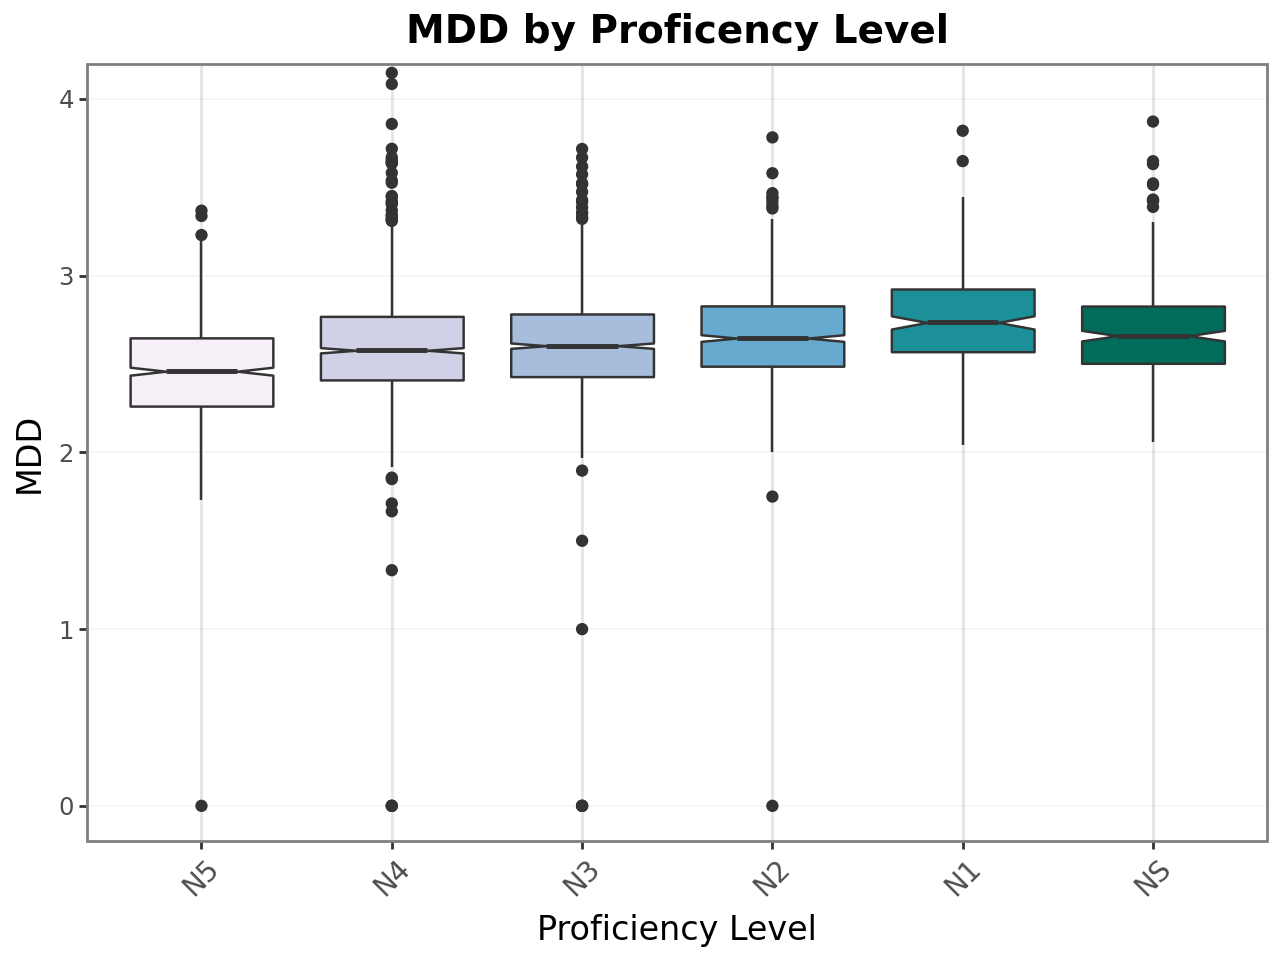
\includegraphics[scale=.4]{img/MDD}
    \caption[Mean Dependency Distance across JLPT Proficency Levels]{Mean Dependency Distance (MDD) increases steadily across JLPT levels, with significant differences between most levels.}
        \label{fig:mdd}
    \end{minipage}
    \hfill
\begin{minipage}{.48\textwidth}
        \centering
        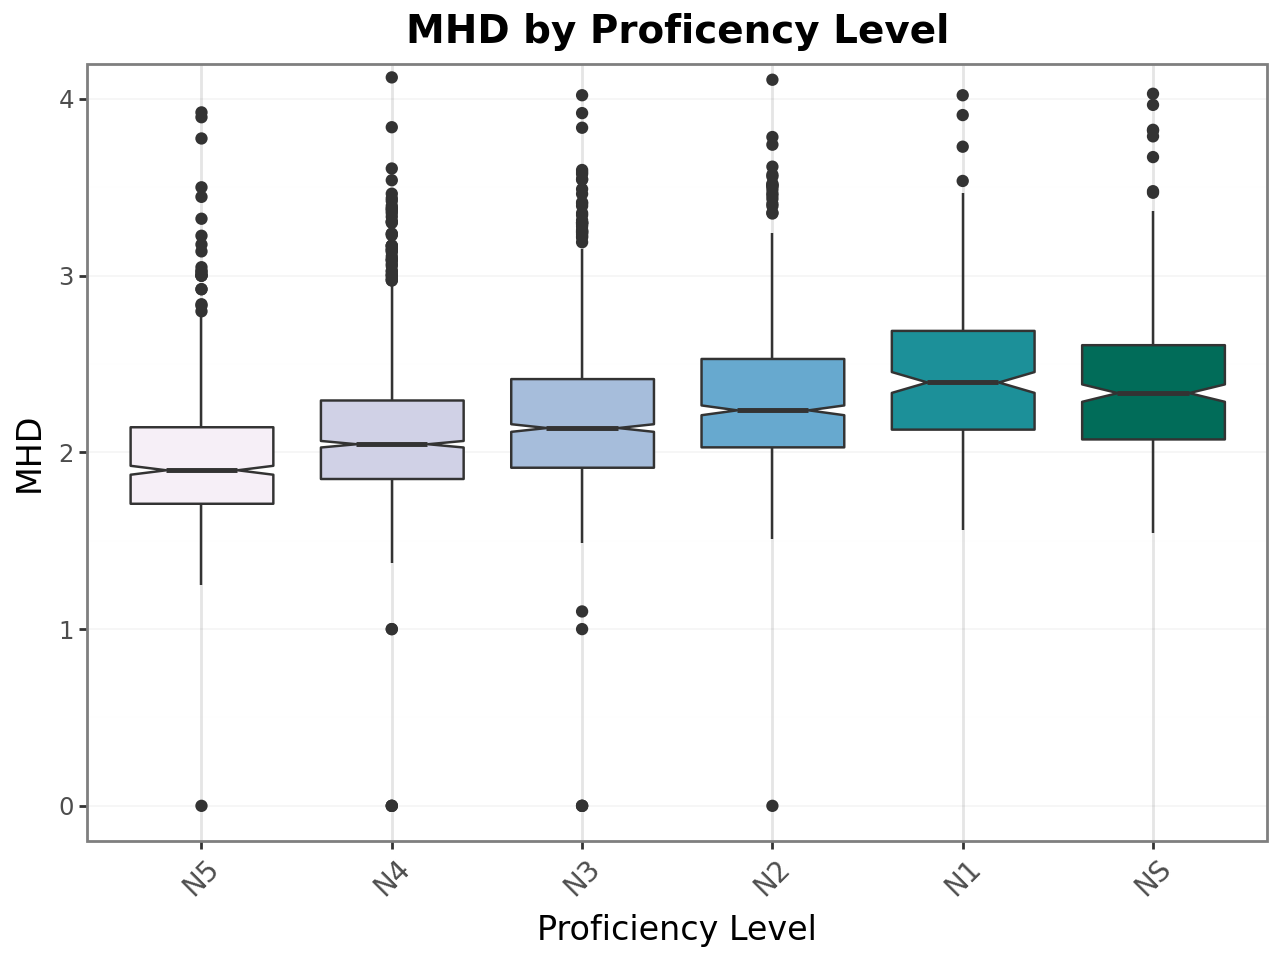
\includegraphics[scale=.4]{img/MHD}
        \caption[Mean Hierarchtical Distance across JLPT Proficency Levels]{Mean Hierarchtical Distance (MHD) increases consistently, distinguishing all adjacent proficency levels.}
\label{fig:mhd}
\end{minipage}
    \end{figure}


\subsection{Lexical Complexity Measures}
Lexical complexity captures the diversity, sophistication and density of vocabulary used by learners. The measures
included to evaluate how vocabulary use changes across proficiency levels include type-based diversity metrics, part
-of-speech (POS) density ratios, and lexical frequency profiles.

\subsubsection{Lexical Diversity Measures}
%CTTR
%    *Discriminates between adjacent levels at the lower proficiency levels,but no statistical significant difference
%    found between N2 & N1 and N1 & NS, and N2 and NS
%    *Generally increases between levels

The Corrected Type-Token Ratio (CTTR) showed a general increase across proficiency levels but was most effective at
distinguishing between adjacent levels in the lower proficiency range (Figure~\ref{fig:cttr}). No statistically significant
differences were
found between N2 vs. N1. This suggests that CTTR may plateau at advanced levels and is more sensitive to early
vocabulary expansion.

\begin{figure}[h]
    \centering
    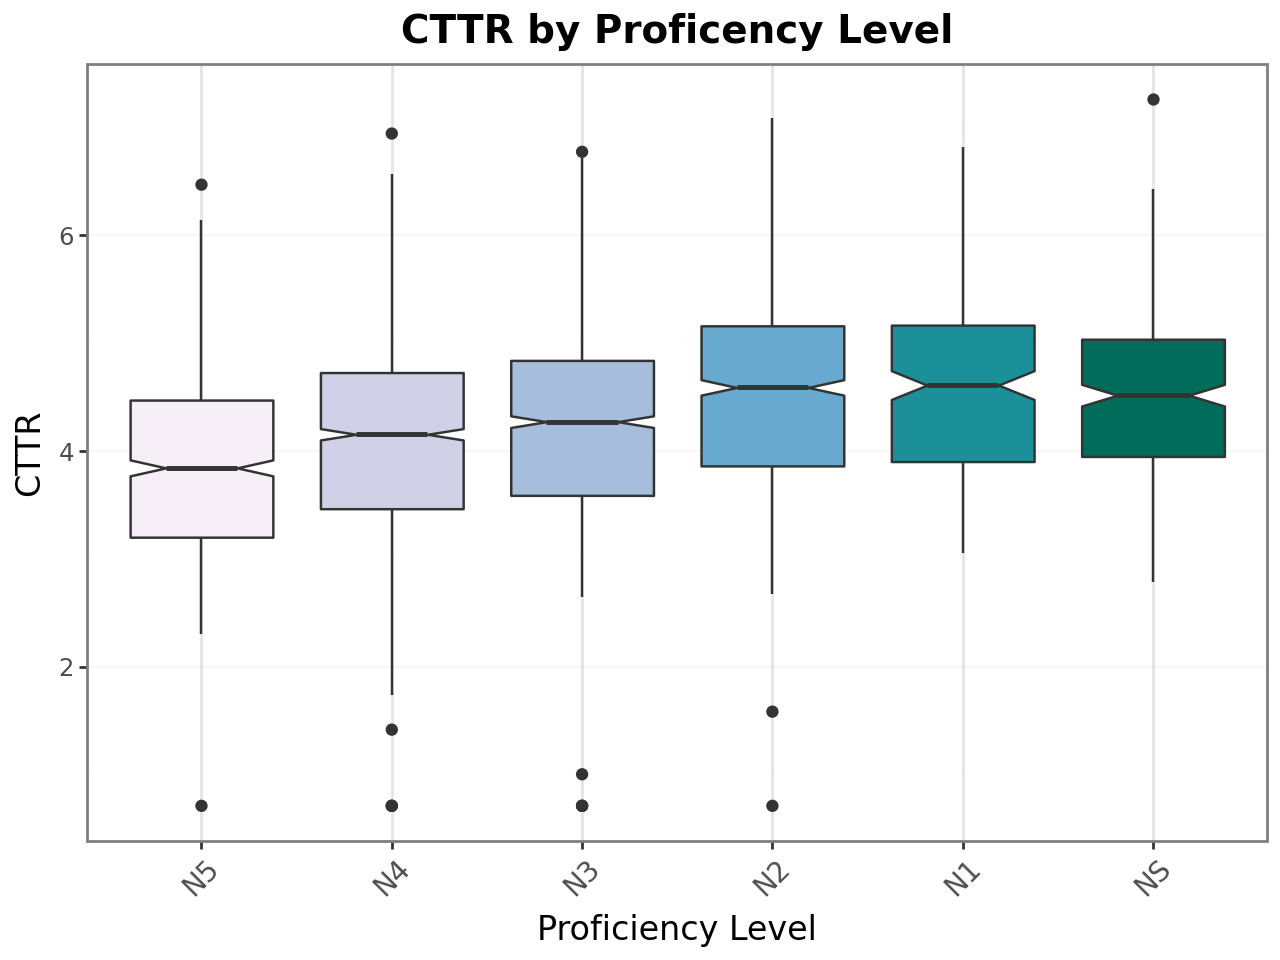
\includegraphics[scale=.5]{img/CTTR}
    \caption[Correct-Type]{CTTR}
    \label{fig:cttr}
\end{figure}

%MTLD-Surface
    %* increases across levels
    %* Statistically significant in distinguishing between lower prof levels.('N2', 'N3'), ('N2', 'N4'), ('N3', 'N5')
%, ('N4','N5')
%MTLD-Inflection
    %*increases across levels not as much as with surface forms
    %* Statistically significant in distinguishing between lower prof levels.('N2', 'N3'), ('N2', 'N4'), ('N3', 'N5')
%, ('N4','N5')

The Measure of Textual Lexical Diversity was calculated for surface forms and lemmas (non-inflected forms). The
MTLD-surface measure increased steadily across proficiency levels and showed statistically significant differences
for several adjacent pairs in the lower and mid-proficiency ranges (N5 vs. N4, N3 vs. N2). This suggest a gradual
increase in word variety as learners develop their langauge (Figure~\ref{fig:mtldS}). The MTLD-lemma measure also
showed an increasing trend, although the effect size was smaller than for surface forms(Figure~\ref{fig:mtldL}). Statistically
significant
differences were observed between similar level pairs, suggesting that while learners increase their morphological
variation, this dimension of diversity develops more slowly.


\begin{figure}[htbp]
    \centering
    \begin{minipage}{.48\textwidth}
        \centering
    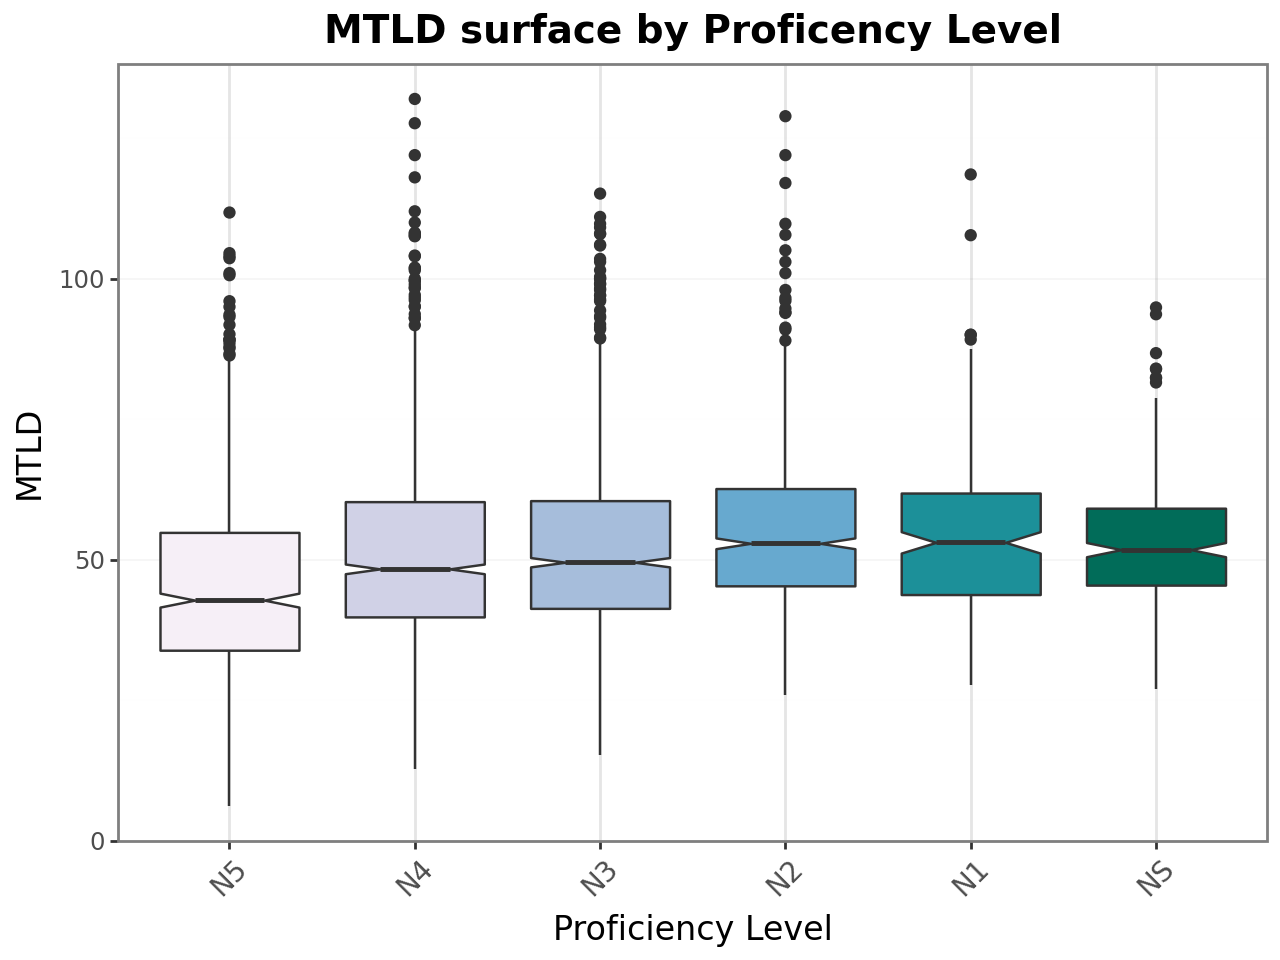
\includegraphics[scale=.4]{img/MTLDsurface}
    \caption[MTLD Surface]{MTLD Surface}
        \label{fig:mtldS}
    \end{minipage}
    \hfill
\begin{minipage}{.48\textwidth}
        \centering
        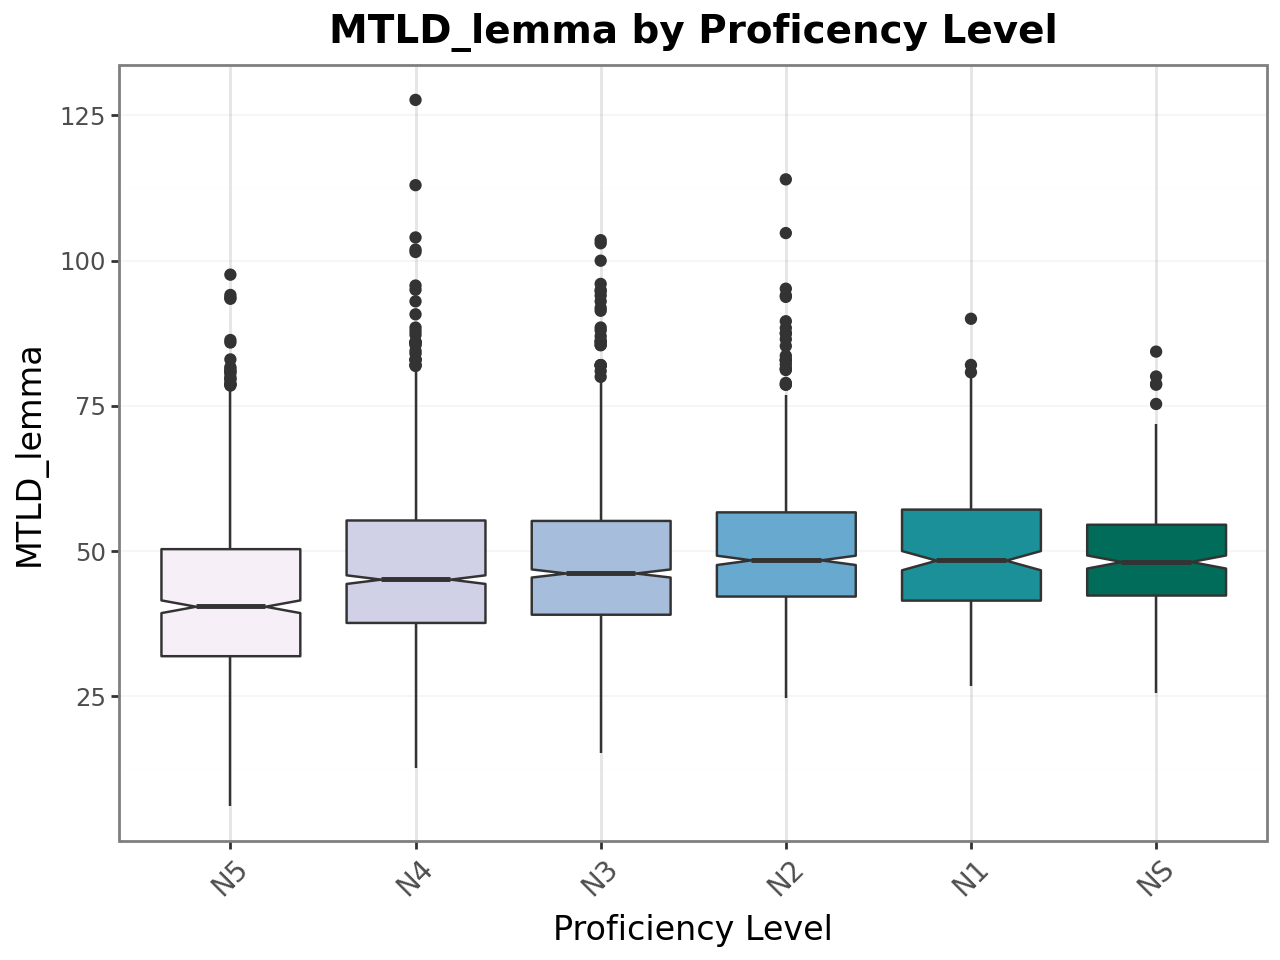
\includegraphics[scale=.4]{img/MTLDlemma}
        \caption[MTLD lemma]{MTLD Lemma}
\label{fig:mtldL}
\end{minipage}
    \end{figure}

\subsubsection{Lexical Density Measures}

Part-of-speech density ratios provide insight into how learners balance content and function words in their writing.
These ratios were normalized by total token count
%Noun Density
    %*Decreases across proficiency levels (null subjects?)
    %*distinguishes beteween lower prof levels. N4 & N5 and N3 and N4 (almost significant p = .06)
%Verb Density
    %*increase across levels
    %* Only statistically significant at distinguishing between lower levels N5 & N4 and N4&N3
Noun density decreased across proficiency levels. This may partially be explained by the use of null subjects in
Japanese, leading to fewer overt noun phrases in more advanced writing (Figure~\ref{fig:nounDen}). Statistically significant
differences were
observed between N5-N4 and N4-N3.

Verb density increased with proficiency but plateaued at the more advanced levels (Figure~\ref{fig:verbDen}) and was only
statistically
significant in distinguishing between the lower adjacent levels (N5-N4 and N4-N3). This pattern suggents that while
verb use expands early, it stabilizes in the upper ranges.

\begin{figure}[htbp]
    \centering
    \begin{minipage}{.48\textwidth}
        \centering
    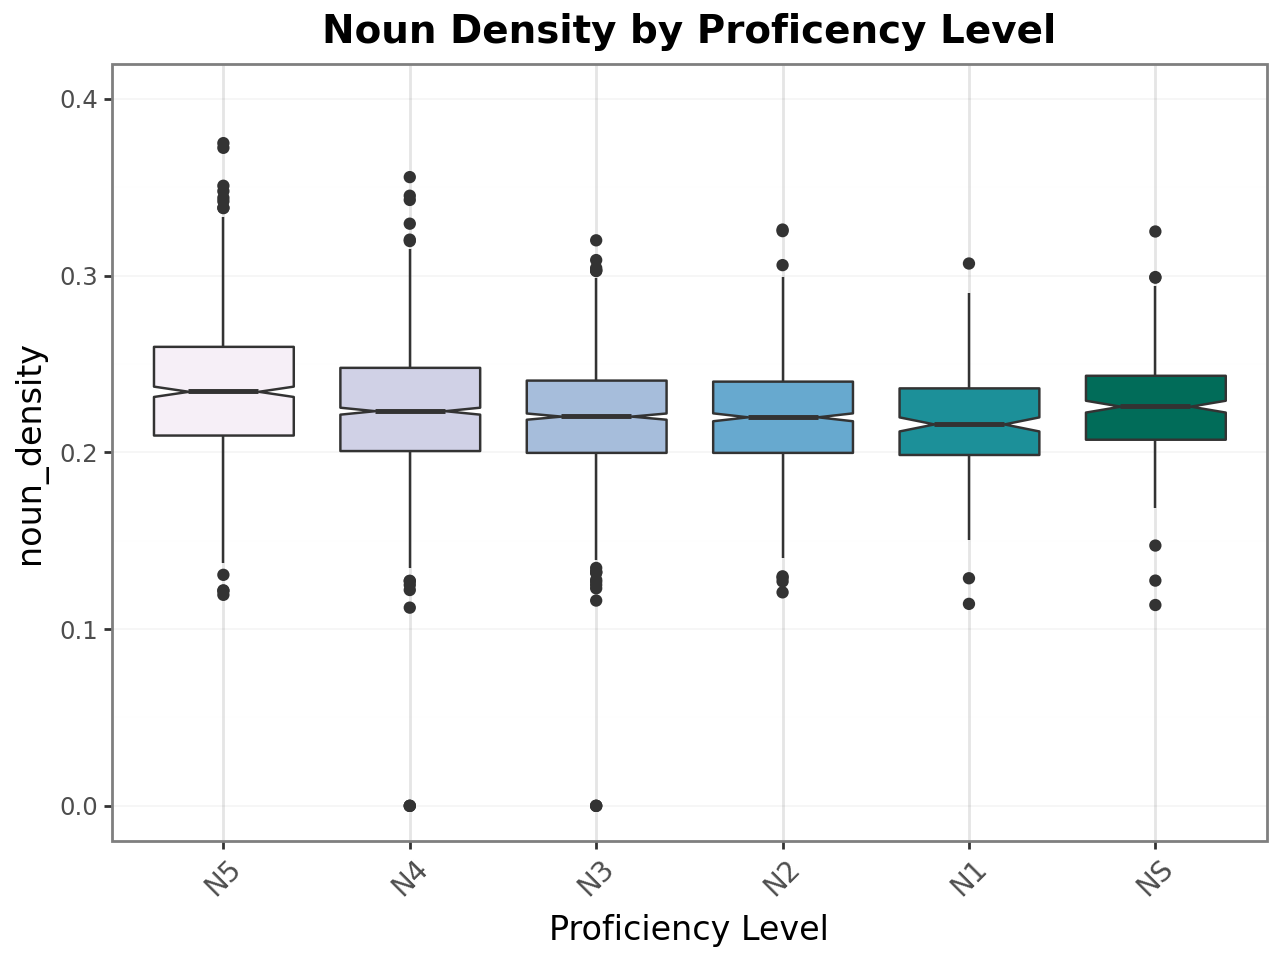
\includegraphics[scale=.4]{img/NounDen}
    \caption[Noun Density Across JLPT Proficiency Levels]{Noun Density}
        \label{fig:nounDen}
    \end{minipage}
    \hfill
\begin{minipage}{.48\textwidth}
        \centering
        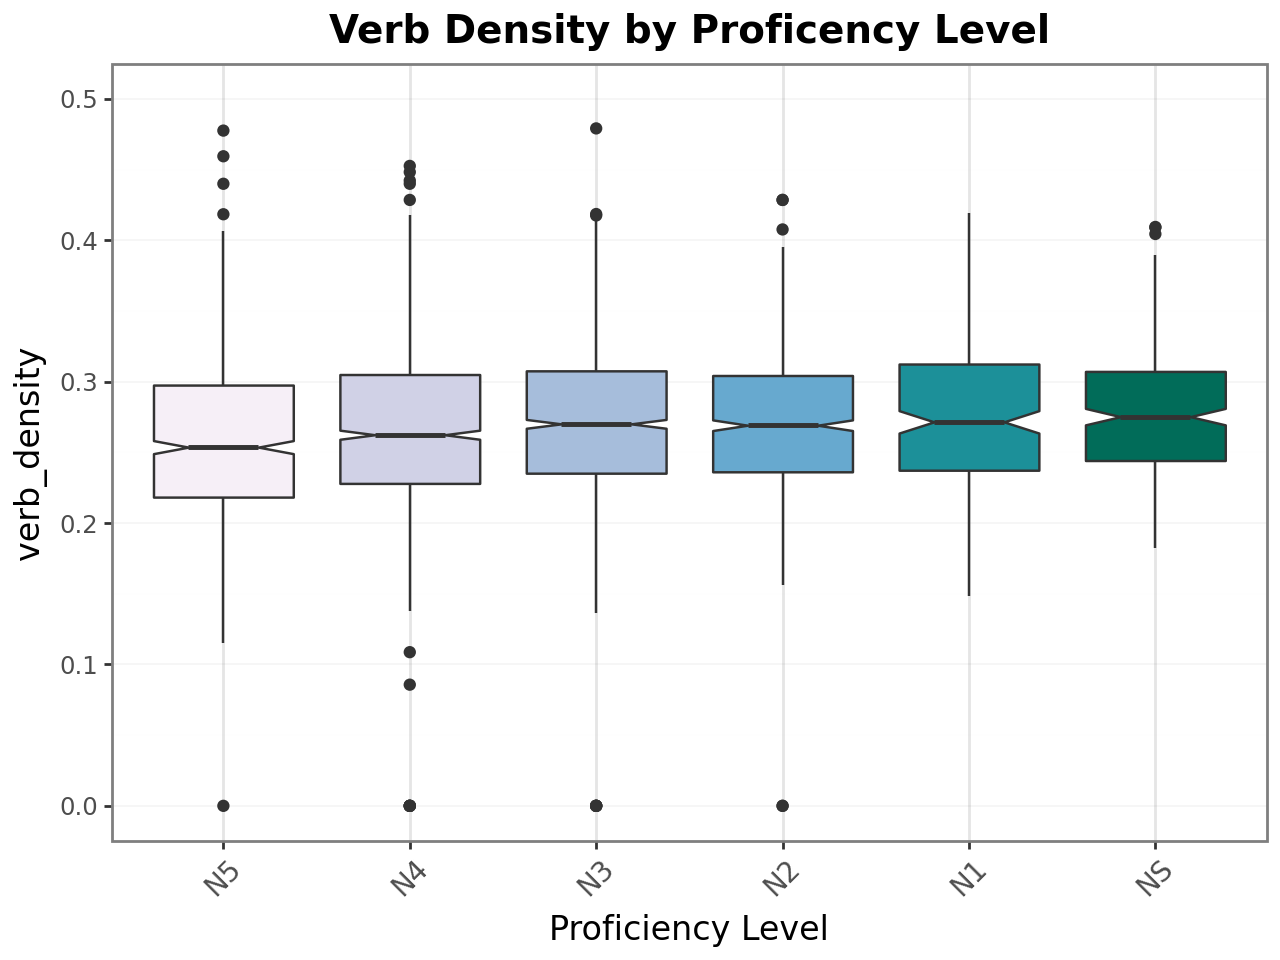
\includegraphics[scale=.4]{img/VerbDen}
        \caption[Verb Density Across JLPT Proficiency Levels]{Verb Density}
\label{fig:verbDen}
\end{minipage}
    \end{figure}


%Adjective Density
    %*Increase across proficiency levels
    %*Statistically significant in distinguishing between lower levels N5&N4, N5&N3, N3&N2
    %*could also be task dependent check later
%Adverb Density
    %*increase across levels except a drop in use for N1 (due to low sample size?)
    %*Statistically significant in distinguishing between lower levels N4&N5, N3&N5 N3&N2
Adjective density showed a consistent increase across proficiency levels and was statistically significant in
distinguishing lower and intermediate pairs (N5-N4, N5-N3, N3-N2). However, this measure may be task-dependent and
should
be interpreted cautiously.
%TODO - check against task.

Adverb density also increased across levels, though with a noticeable drop at N1. This may be due to sample size
limitations or task variation. Statistically significant differences were found between N5-N4, N5-N3, and N3-N2,
indicating usefulness in assessment of early-stage proficiency.

\begin{figure}[htbp]
    \centering
    \begin{minipage}{.48\textwidth}
        \centering
    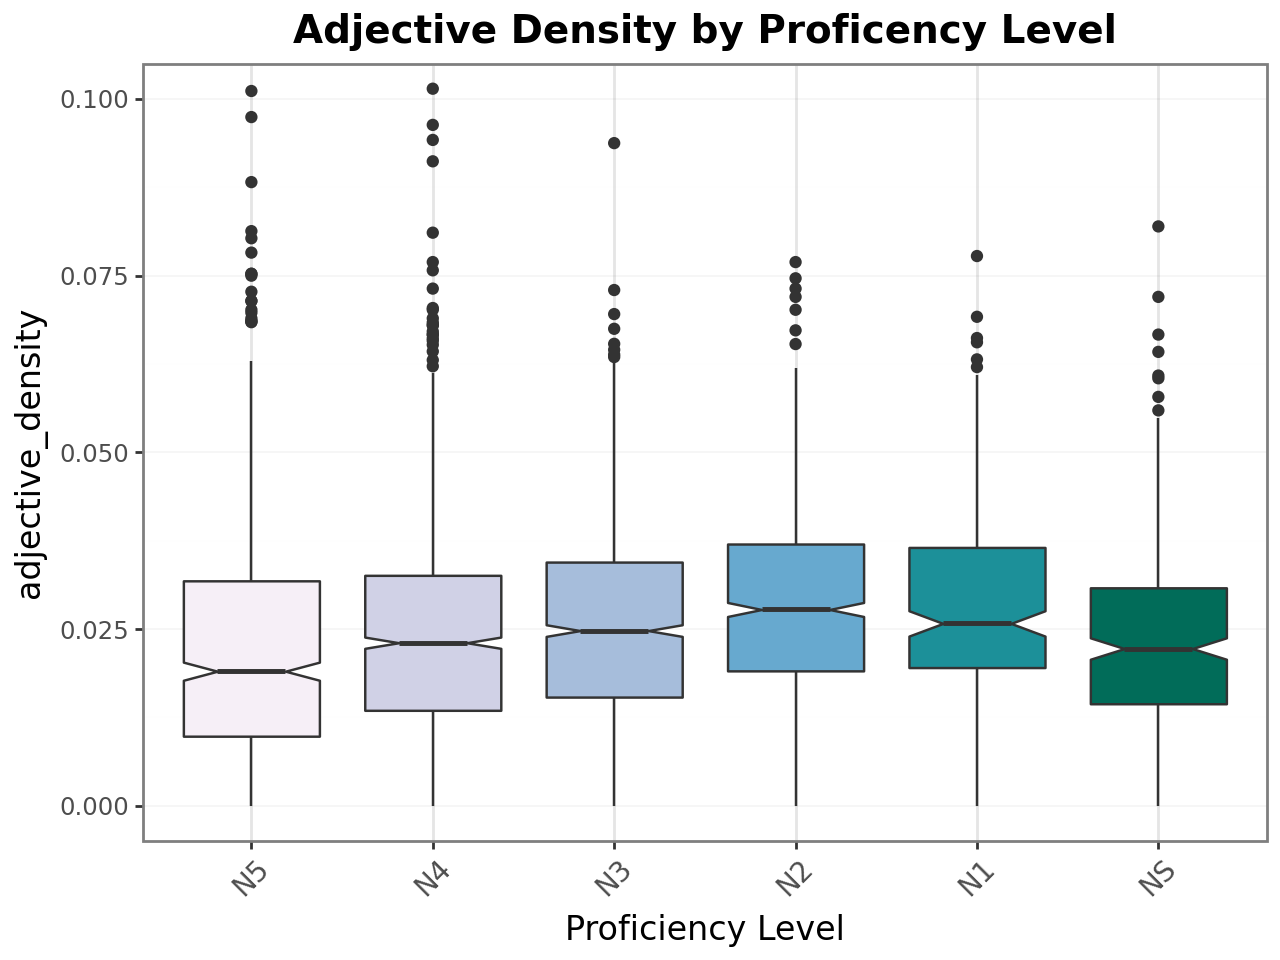
\includegraphics[scale=.4]{img/AdjDen}
    \caption[Adjective Density Across JLPT Proficiency Levels]{Adjective Density}
        \label{fig:adjDen}
    \end{minipage}
    \hfill
\begin{minipage}{.48\textwidth}
        \centering
        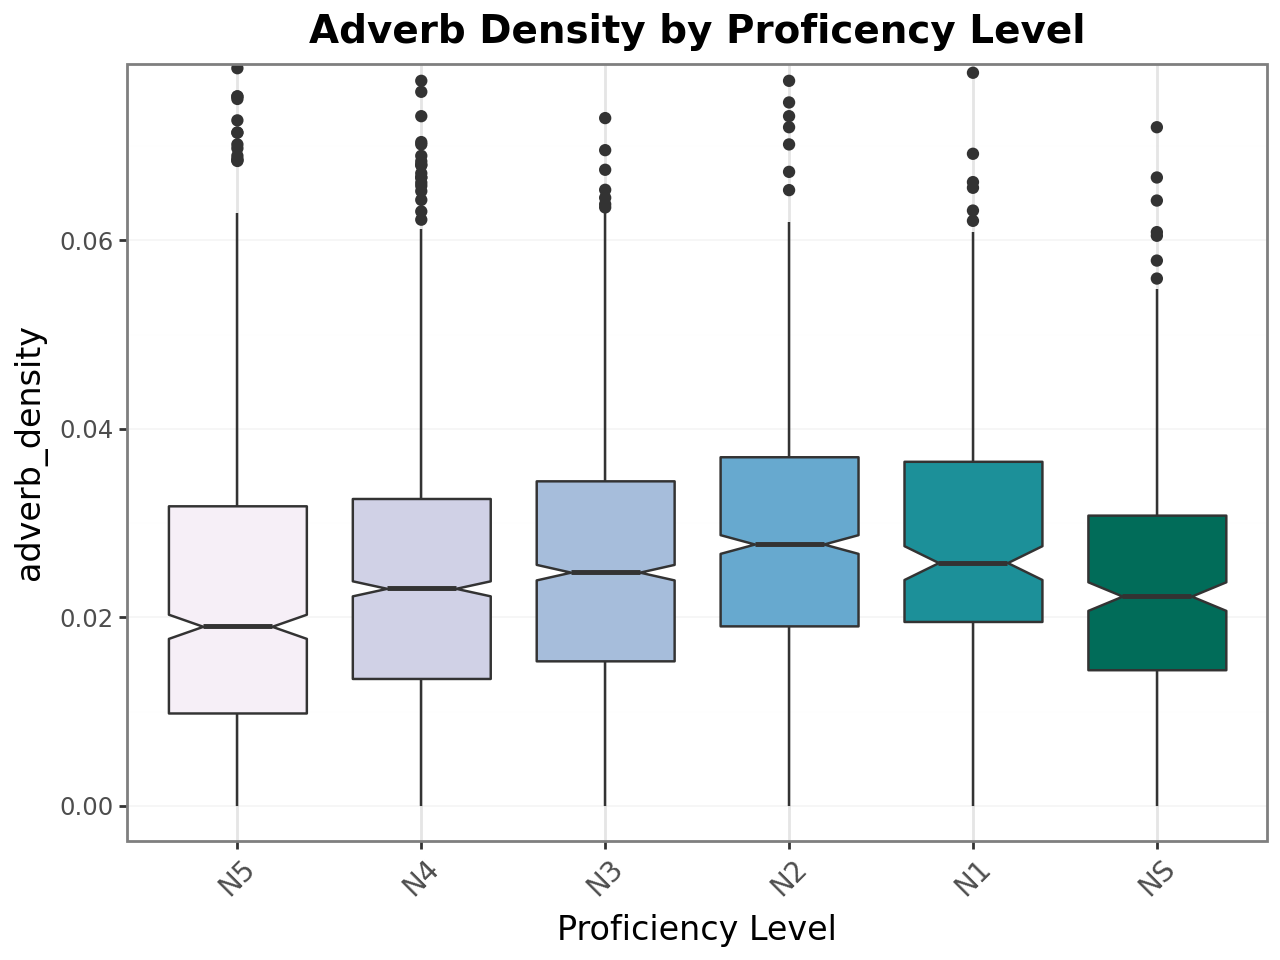
\includegraphics[scale=.4]{img/AdvDen}
        \caption[Adverb Density Across JLPT Proficiency Levels]{Adverb Density}
\label{fig:advDen}
\end{minipage}
    \end{figure}

\subsubsection{Lexical Frequency Profile Measures}
The Lexical Frequency Profile (LFP) was calculated using two difference reference corpora: the Balanced Corpus of
Contemporary Written Japanese (BCCWJ) \citep{maekawa2014} and a JLPT-aligned wordlist.

LFP

LFP -BWCCJ Corpus
    * high frequency of items in top 1,000 band across all proficiency levels
    *N1 and Ns group had the largest raw count of vocab used across each band
    * However,

LFP - JLPT WordList
    *

\subsection{Morphological}
*MCI - Surface vs. Lemma
\subsubsection{MCI Measures}
MCI 5-Surface
\begin{itemize}
   \item *46 texts removed
   \item  *Increase across levels
    \item *statistically significant across groups except N1&NS and N1 and N2
 \end{itemize}
MCI 5-Inflection
    *46 texts dropped
    *not as great an increase across levels
    *does not discriminate between adjacent levels but every other level at lower levels N5&N3, N4&N2
MCI 10 - Surface (634 texts dropped)
    * Increase across levels
    * Statistically significant at lower levels N5 - N2 , no significance between N2, N1, NS
MCI 10 - Inflection
    *statistically significant difference between N1 and NS!
    *Statistically significant at lower levels N5-N2, no significance between N2 and N1

*Conclusion the surface/standard calculation is enough and yields more statistically significant results.MCI10
results in more learner texts being dropped due to length. MCI5 is more than enough when working with lower
proficiency learners.
\subsubsection{JRMA Measures}
JRMA Measures

*MTLD measures had dropped texts due to the minimum text length limit required. This is especially true for
these measures as it is using specific function/content words meaning even longer text is needed.


JRMA_all_MTLD
    *49 rows removed
    *statistically significant difference in distinguishing N5&N4, N3&N2 levels

JRMA_function_MTLD
    *2377 rows removed
    * only difference in N4 and N3 were statistically significant.
    *no clear pattern of increasing/decreasing

JRMA_content_MTLD
    * 2446 rows removed of 4840
    * Statistically significant in distinguishing the lower levels. N4&N5 N3&N2
*
JRMA_all_MATTR
    *Significant difference between all levels except the N1&NS,and N1&N2
    * slight increase across levels, variance also decreases

JRMA_Function_MATTR
    *Slight decrease across levels.
    *decrease in variance across levels
    * significant pairs: (N5,N4), (N4,N3),(N5,N3)

JRMA_Content_MATTR
    * decrease in variance across levels
    * significant pairs: (N2,N3), (N5,N3)

Auxiliary Chains
    * significant pairs (N5,N4),(N3,N5)
    * increase from N5 to N4, but after that plateaus. Meaning that after the beginning levels chain size doesn't
    increase

\subsubsection{Summary}
Write here summarizing the most demonstrative complexity measures:
i.e. Syntactic: Sent Length,Coordinate Clauses per sentence,  MDD, MHD

Lexical: CTTR over MTLD?

Morphological:


\section{Criterial Features}
Raw counts of features, 
look at how many of structures from each level are used across all features used


possibly also include qualitative analysis on extracted grammar forms.?

Raw counts of grammar forms across all proficency levels (and native)

CF_tai_N5_total          1705
CF_ukemi_N4_total        1688
CF_toomou_N4_total       1586
CF_toiu_N3_total         1056
CF_tara_N4_total          948
CF_youni_N4_total         822
CF_tabini_N3_total        520
CF_tekudasai_N5_total     495
CF_saseru_N4_total        471
CF_tekuru_N4_total        333

\section{Task Effect}
Look into differences in results across tasks...